\documentclass[10pt,a4paper]{article}
\usepackage[margin=1.6cm]{geometry}
\usepackage{graphicx,booktabs,amsmath,hyperref}
\graphicspath{{figures/}{../figures/}}
\setlength{\parskip}{0.28em}
\setlength{\parindent}{0pt}
\setlength{\textfloatsep}{4pt plus 1pt minus 2pt}
\setlength{\floatsep}{4pt plus 1pt minus 2pt}
\setlength{\intextsep}{4pt plus 1pt minus 2pt}
\setlength{\abovecaptionskip}{3pt}
\setlength{\belowcaptionskip}{0pt}
\hypersetup{colorlinks=true,urlcolor=black}
\pagestyle{plain}

\begin{document}
\begin{center}
{\large\bfseries Survival groups after pediatric bone-marrow transplantation}\\[0.15em]
Lukas Juranek\\[0.1em]
{\footnotesize Lab II, Machine Learning in Health \quad November 2026}
\end{center}
\vspace{-0.35em}

\noindent
The UCI bone-marrow cohort has 187 children who received an unmanipulated allogeneic transplant (85 deaths, 102 censored; follow-up 6--3364 days). The scientific question attached to the file is whether a higher CD34+ cell dose lengthens survival. This analysis asks a related question: do baseline features form patient groups with different survival, and do Kaplan--Meier and Cox regression tell the same story?

\textbf{Methods.}
Predictors are restricted to information known at transplant. Relapse, GvHD, and neutrophil or platelet recovery are excluded. Those recovery and GvHD-time columns also use the sentinel value \(10^6\), which would otherwise dominate any distance. Twelve attributes have missing values (45 patients; worst is extensive chronic GvHD, 31). Median or modal imputation is used for clustering. Association with survival is a univariate Cox model, not a Pearson correlation with the observed time, because censoring makes that correlation misleading. Redundant copies are dropped: age bins, the HLA block (Cox keeps a binary mismatch), ABO and CMV detail, and body mass, which tracks recipient age (Spearman \(\rho=0.93\)).

Thirteen baseline inputs are standardized, with disease one-hot encoded, and reduced by PCA to 85\% of variance (11 components, 88.6\%). K-means uses \(K\in\{2,\ldots,8\}\) with 50 restarts. \(K\) maximizes silhouette subject to every cluster having at least 15 patients. Kaplan--Meier curves and a log-rank test compare clusters. Cox model A has eight covariates (85/8 \(\approx 10.6\) events per variable): recipient age per 5 years, donor age per 10 years, log CD34 dose, malignant disease, high risk, second transplant, HLA mismatch, and peripheral-blood stem cells. Model B adds cluster indicators (largest cluster as reference). Proportional hazards are checked with rank-transformed Schoenfeld tests. Discrimination is Harrell's C-index, including 5-fold cross-validation with the imputer fit inside each fold. A ridge Cox on the full clustering design (model C) is used only to check coefficient signs.

\textbf{Results.}
Overall median survival is not reached (the curve levels off near 0.53). Reverse-KM median follow-up is 1522 days. The strongest univariate signals are body mass (HR 1.021 per kg, \(p=3\times 10^{-4}\)), lymphoma versus ALL (HR 3.87, 95\% CI 1.83--8.20; nine patients), CD3+ dose (HR 0.90 per \(10^8\)/kg, \(p=0.002\)), recipient age (HR 1.067 per year, \(p=0.003\)), and CD34+ dose (HR 0.971 per \(10^6\)/kg, \(p=0.035\)). Pearson correlation can disagree: peripheral-blood grafts have Cox HR 0.63 but Pearson \(r=-0.04\) with observed time. Variance inflation factors in model A are all below 2.2.

\begin{figure}[ht]
\centering
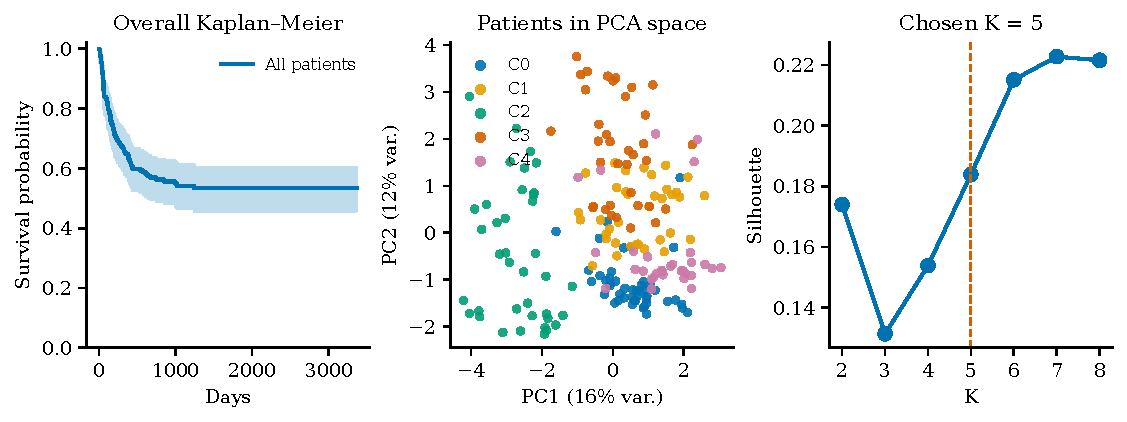
\includegraphics[width=\textwidth]{fig1_overview.pdf}
\caption{Overall Kaplan--Meier, the K-means partition in the first two principal components (27\% of variance), and silhouette. \(K=6\) scores higher but leaves a cluster of size 9, so \(K=5\) (silhouette 0.18).}
\end{figure}

\noindent
The five groups mostly recover diagnosis and graft source, not a hidden risk score (Table~\ref{tab:clusters}). Cluster 2 is almost entirely bone marrow and has a much lower CD34 dose (median 2.9 versus 10--16). Its Kaplan--Meier curve sits below the others (median 421 days versus not reached, or 1243 days in the AML group), but the five-group log-rank test is not significant (\(\chi^2=5.41\), \(p=0.25\)). The only pairwise \(p<0.05\) (ALL versus marrow) becomes 0.49 after Bonferroni.

\begin{table}[ht]
\centering
\footnotesize
\begin{tabular}{@{}clrrrr@{}}
\toprule
& Group & \(n\) & Deaths & Median (days) & CD34 median\\
\midrule
C0 & ALL, low-risk & 46 & 17 & not reached & 10.1\\
C1 & Chronic, poorer HLA match & 36 & 17 & not reached & 11.5\\
C2 & Mostly marrow, lower CD34 & 38 & 22 & 421 & 2.9\\
C3 & AML, often post-relapse & 36 & 18 & 1243 & 10.3\\
C4 & Nonmalignant, younger & 31 & 11 & not reached & 16.0\\
\bottomrule
\end{tabular}
\caption{K-means groups. CD34 dose is \(\times 10^6\) cells/kg.}
\label{tab:clusters}
\end{table}

\begin{figure}[ht]
\centering
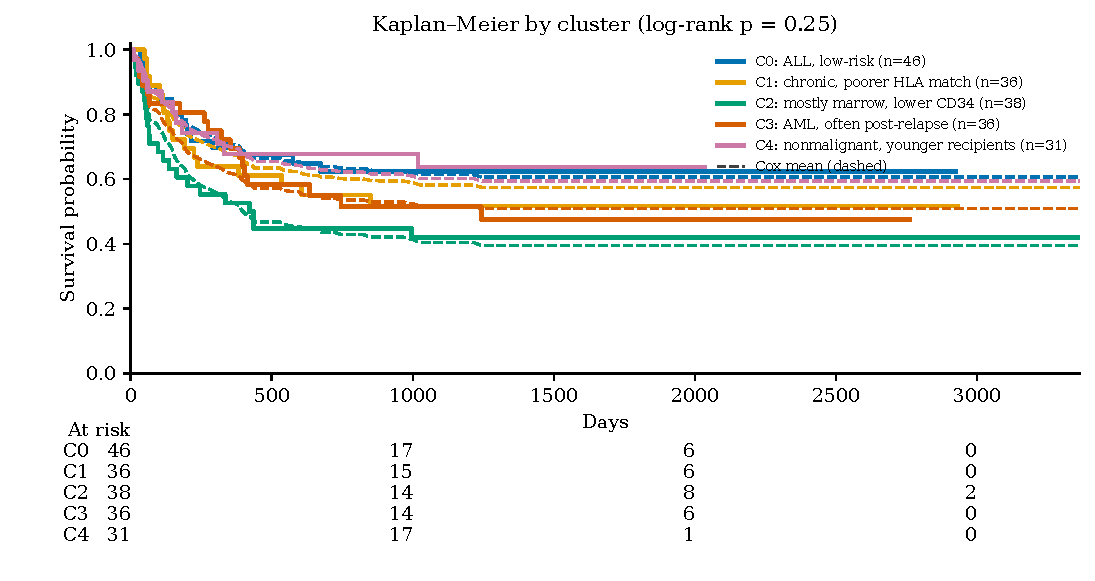
\includegraphics[width=\textwidth]{fig2_km_cox.pdf}
\caption{Solid curves are Kaplan--Meier. Dashed curves are the mean Cox survival in that cluster from model A after stratifying on HLA mismatch. The curves agree; the groups are not separated at \(p=0.25\).}
\end{figure}

\begin{figure}[ht]
\centering
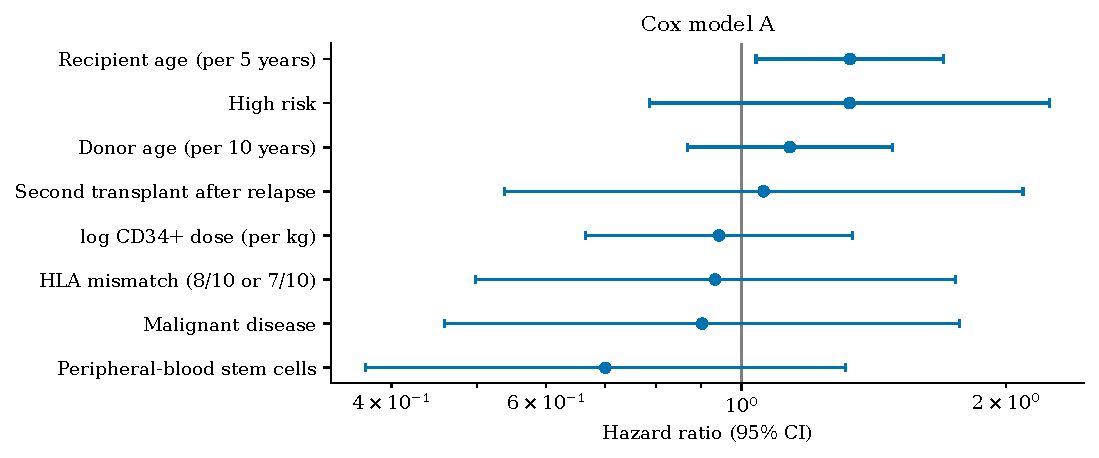
\includegraphics[width=0.92\textwidth]{fig3_forest.pdf}
\caption{Unstratified Cox model A. Only recipient age has a confidence interval that excludes 1 (HR 1.33 per 5 years, 1.04--1.70). Log CD34 dose does not (HR 0.94, \(p=0.74\)).}
\end{figure}

\noindent
Training C-index is 0.61 (0.63 if HLA mismatch is a stratum). Cross-validated C-index is 0.56 (SD 0.04). Adding clusters does not help: likelihood-ratio test \(\chi^2=6.76\) on 4 df, \(p=0.15\), and the cross-validated C-index falls to 0.53. Cluster 4 is exactly the nonmalignant patients, so the disease coefficient and that cluster indicator in model B are not separately interpretable; the joint test is the one to read. Every model C sign matches model A. HLA mismatch is the only proportional-hazards violation at \(p<0.05\) (rank test \(p=0.034\)); stratifying on it leaves the age hazard ratio unchanged. DBSCAN on the same 11 components (\(\varepsilon=5.58\), \(\texttt{min\_samples}=22\), knee of the \(k\)-distance curve) returns one cluster and adjusted Rand index 0 against K-means.

\textbf{Discussion.}
Kaplan--Meier describes each group without assuming proportional hazards, but it does not adjust for covariates and, with 85 events split five ways, it has little power. Cox adjusts and supplies hazard ratios, at the cost of a proportional-hazards assumption that already fails for HLA mismatch. Here the two methods agree: the marrow/low-CD34 group looks worse, the Cox averages sit on the Kaplan--Meier curves, and neither the log-rank test nor the likelihood-ratio test supports a survival difference beyond the covariates. The CD34 hypothesis appears in the univariate screen and then disappears once graft source and the other baseline factors are in the model, which is expected if dose and marrow versus blood are the same contrast. Age is the one signal that survives adjustment.

The clustering itself is a weak partition (silhouette 0.18; two components show 27\% of the variance) and is dominated by one-hot disease indicators: a limit of Euclidean K-means on mixed data, not a new phenotype. Other limits are single imputation, no external cohort, no integrated Brier score, and informative missingness. Patients missing extensive chronic GvHD survive far worse (\(p\sim 10^{-70}\)), because early deaths never reach that endpoint; those fields were not covariates.

\noindent
\textit{Code.} \texttt{notebooks/lab2\_survival.ipynb} in the accompanying repository.

\end{document}
